% Requires graphicx. Paths assume compilation from Manuscript/.
% Captions describe working-set analyses, not final inclusion/prevalence estimates.
\begin{figure*}[t]
\centering
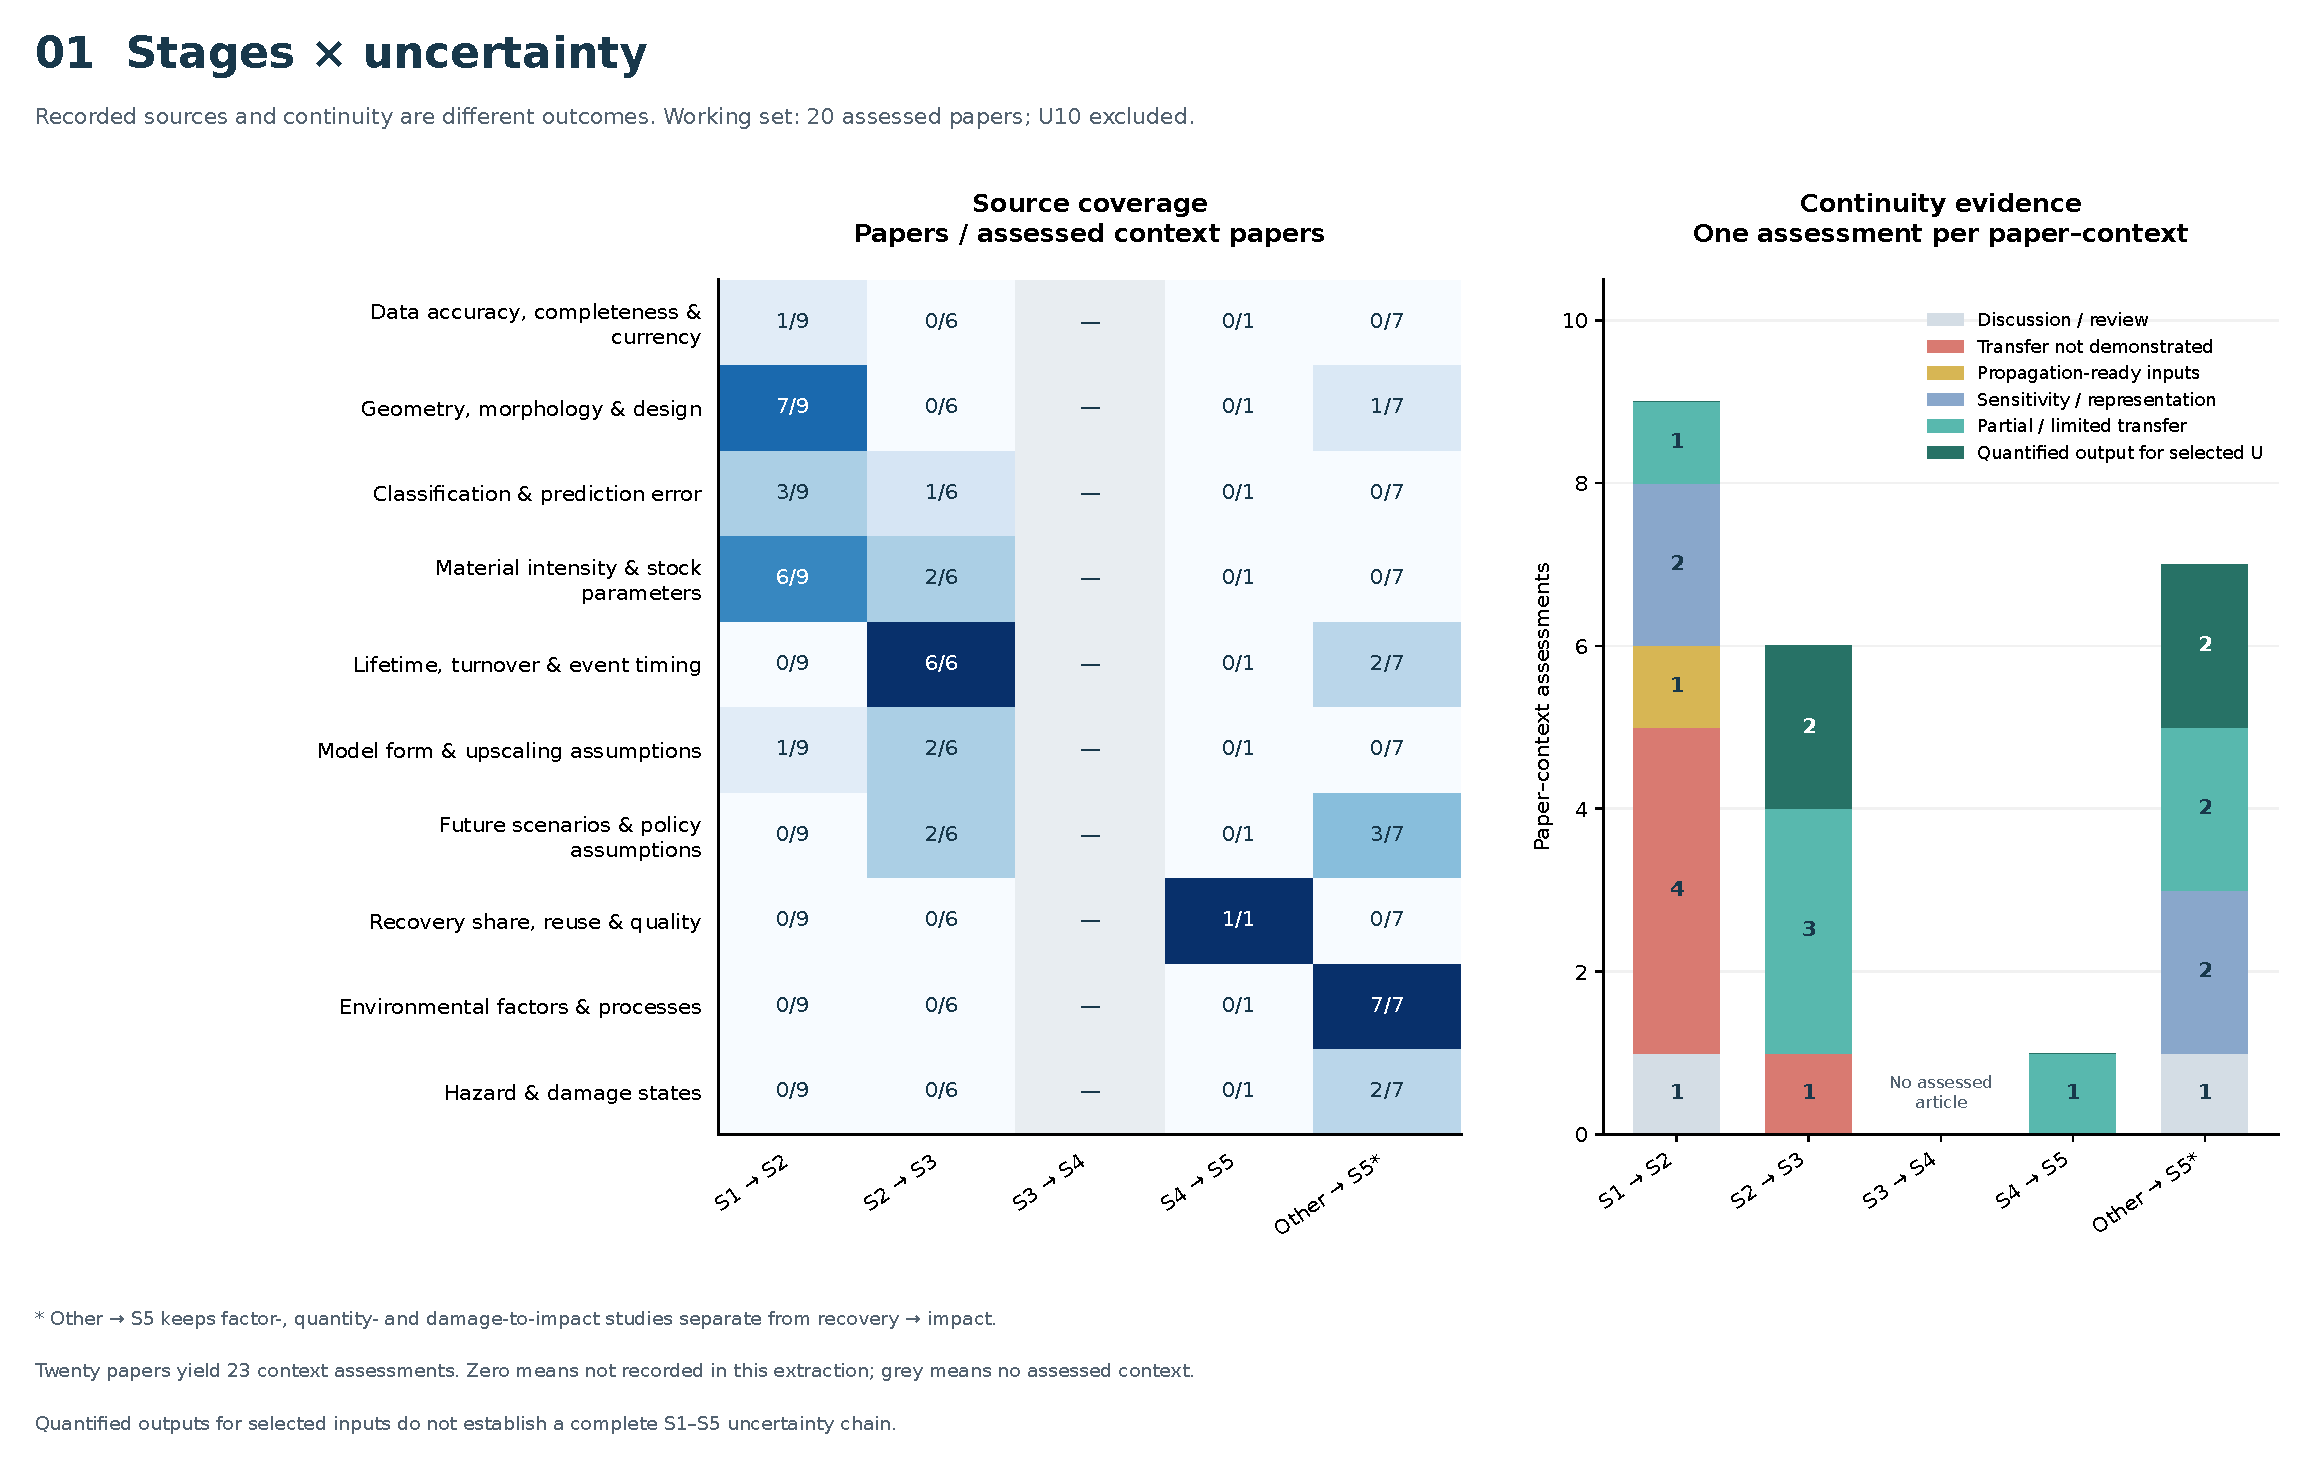
\includegraphics[width=\textwidth]{relational_analysis/results/figures/01_stages_uncertainty.pdf}
\caption{Uncertainty-source coverage and continuity assessments across material-flow boundaries. Twenty assessed publications generate 23 publication--context assessments. Numerators and denominators are shown explicitly; grey denotes an unassessed boundary in the selected set. Other-to-S5 contexts are retained separately from recovery-to-impact transfer.}
\label{fig:relational-su}
\end{figure*}

\begin{figure*}[t]
\centering
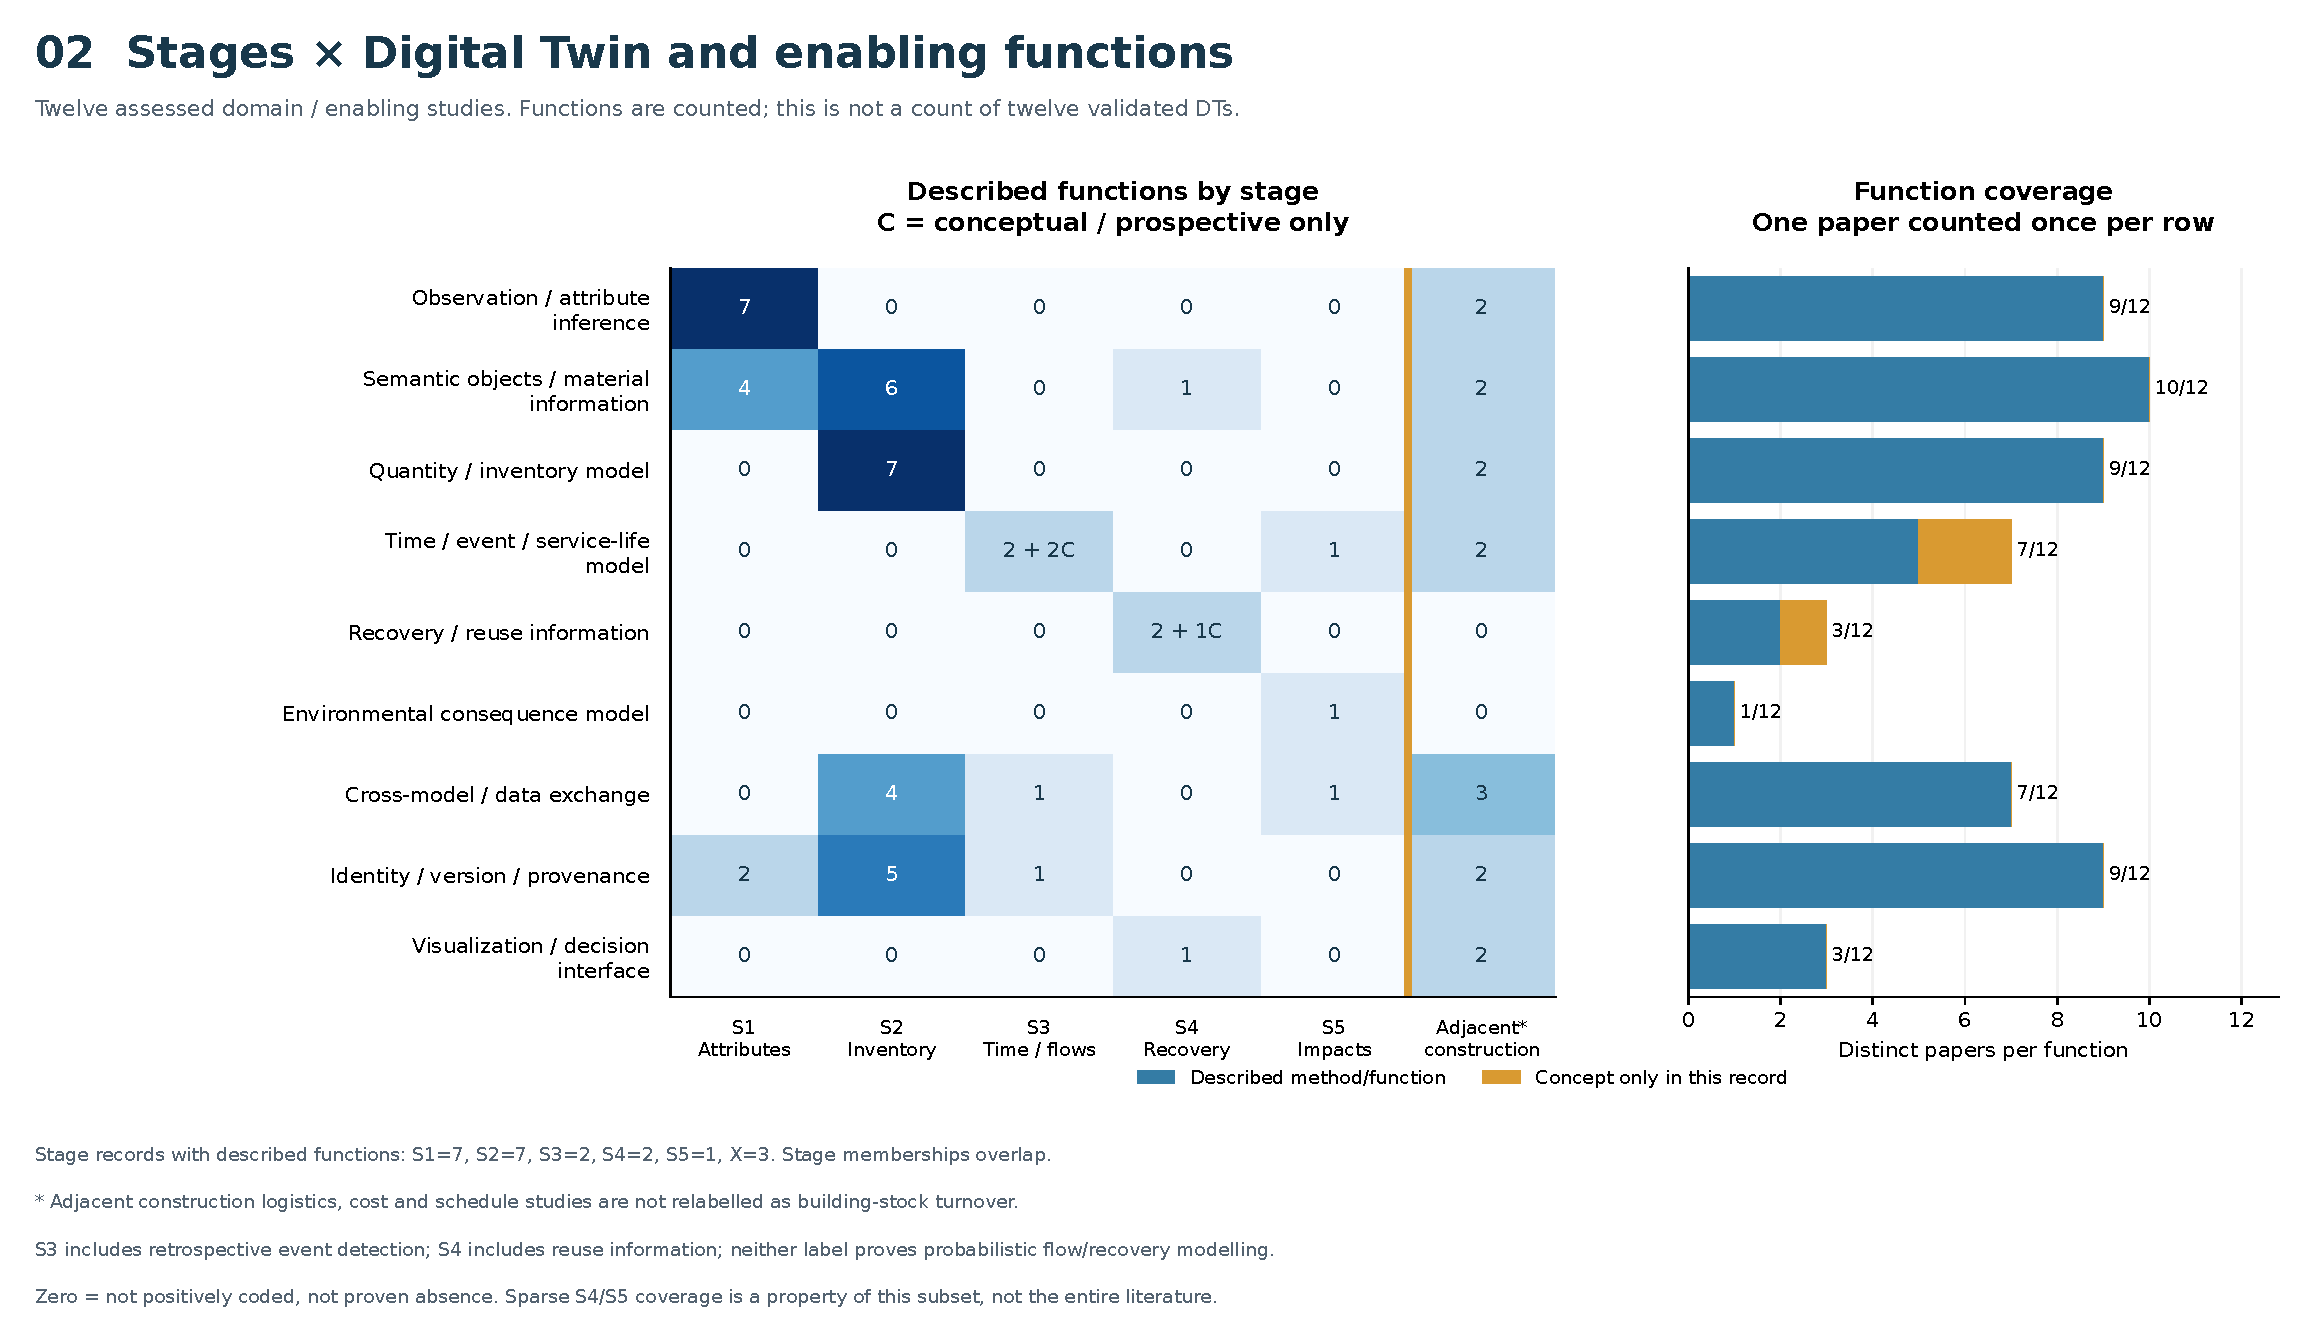
\includegraphics[width=\textwidth]{relational_analysis/results/figures/02_stages_dt_functions.pdf}
\caption{Material-flow stages and domain Digital Twin/enabling functions in twelve assessed publications. Cells count described functions; conceptual or prospective codes are separately marked C. The adjacent category preserves construction, cost and scheduling applications without relabelling them as stock turnover. Memberships overlap and counts do not establish complete DT implementations.}
\label{fig:relational-sdt}
\end{figure*}

\begin{figure*}[t]
\centering
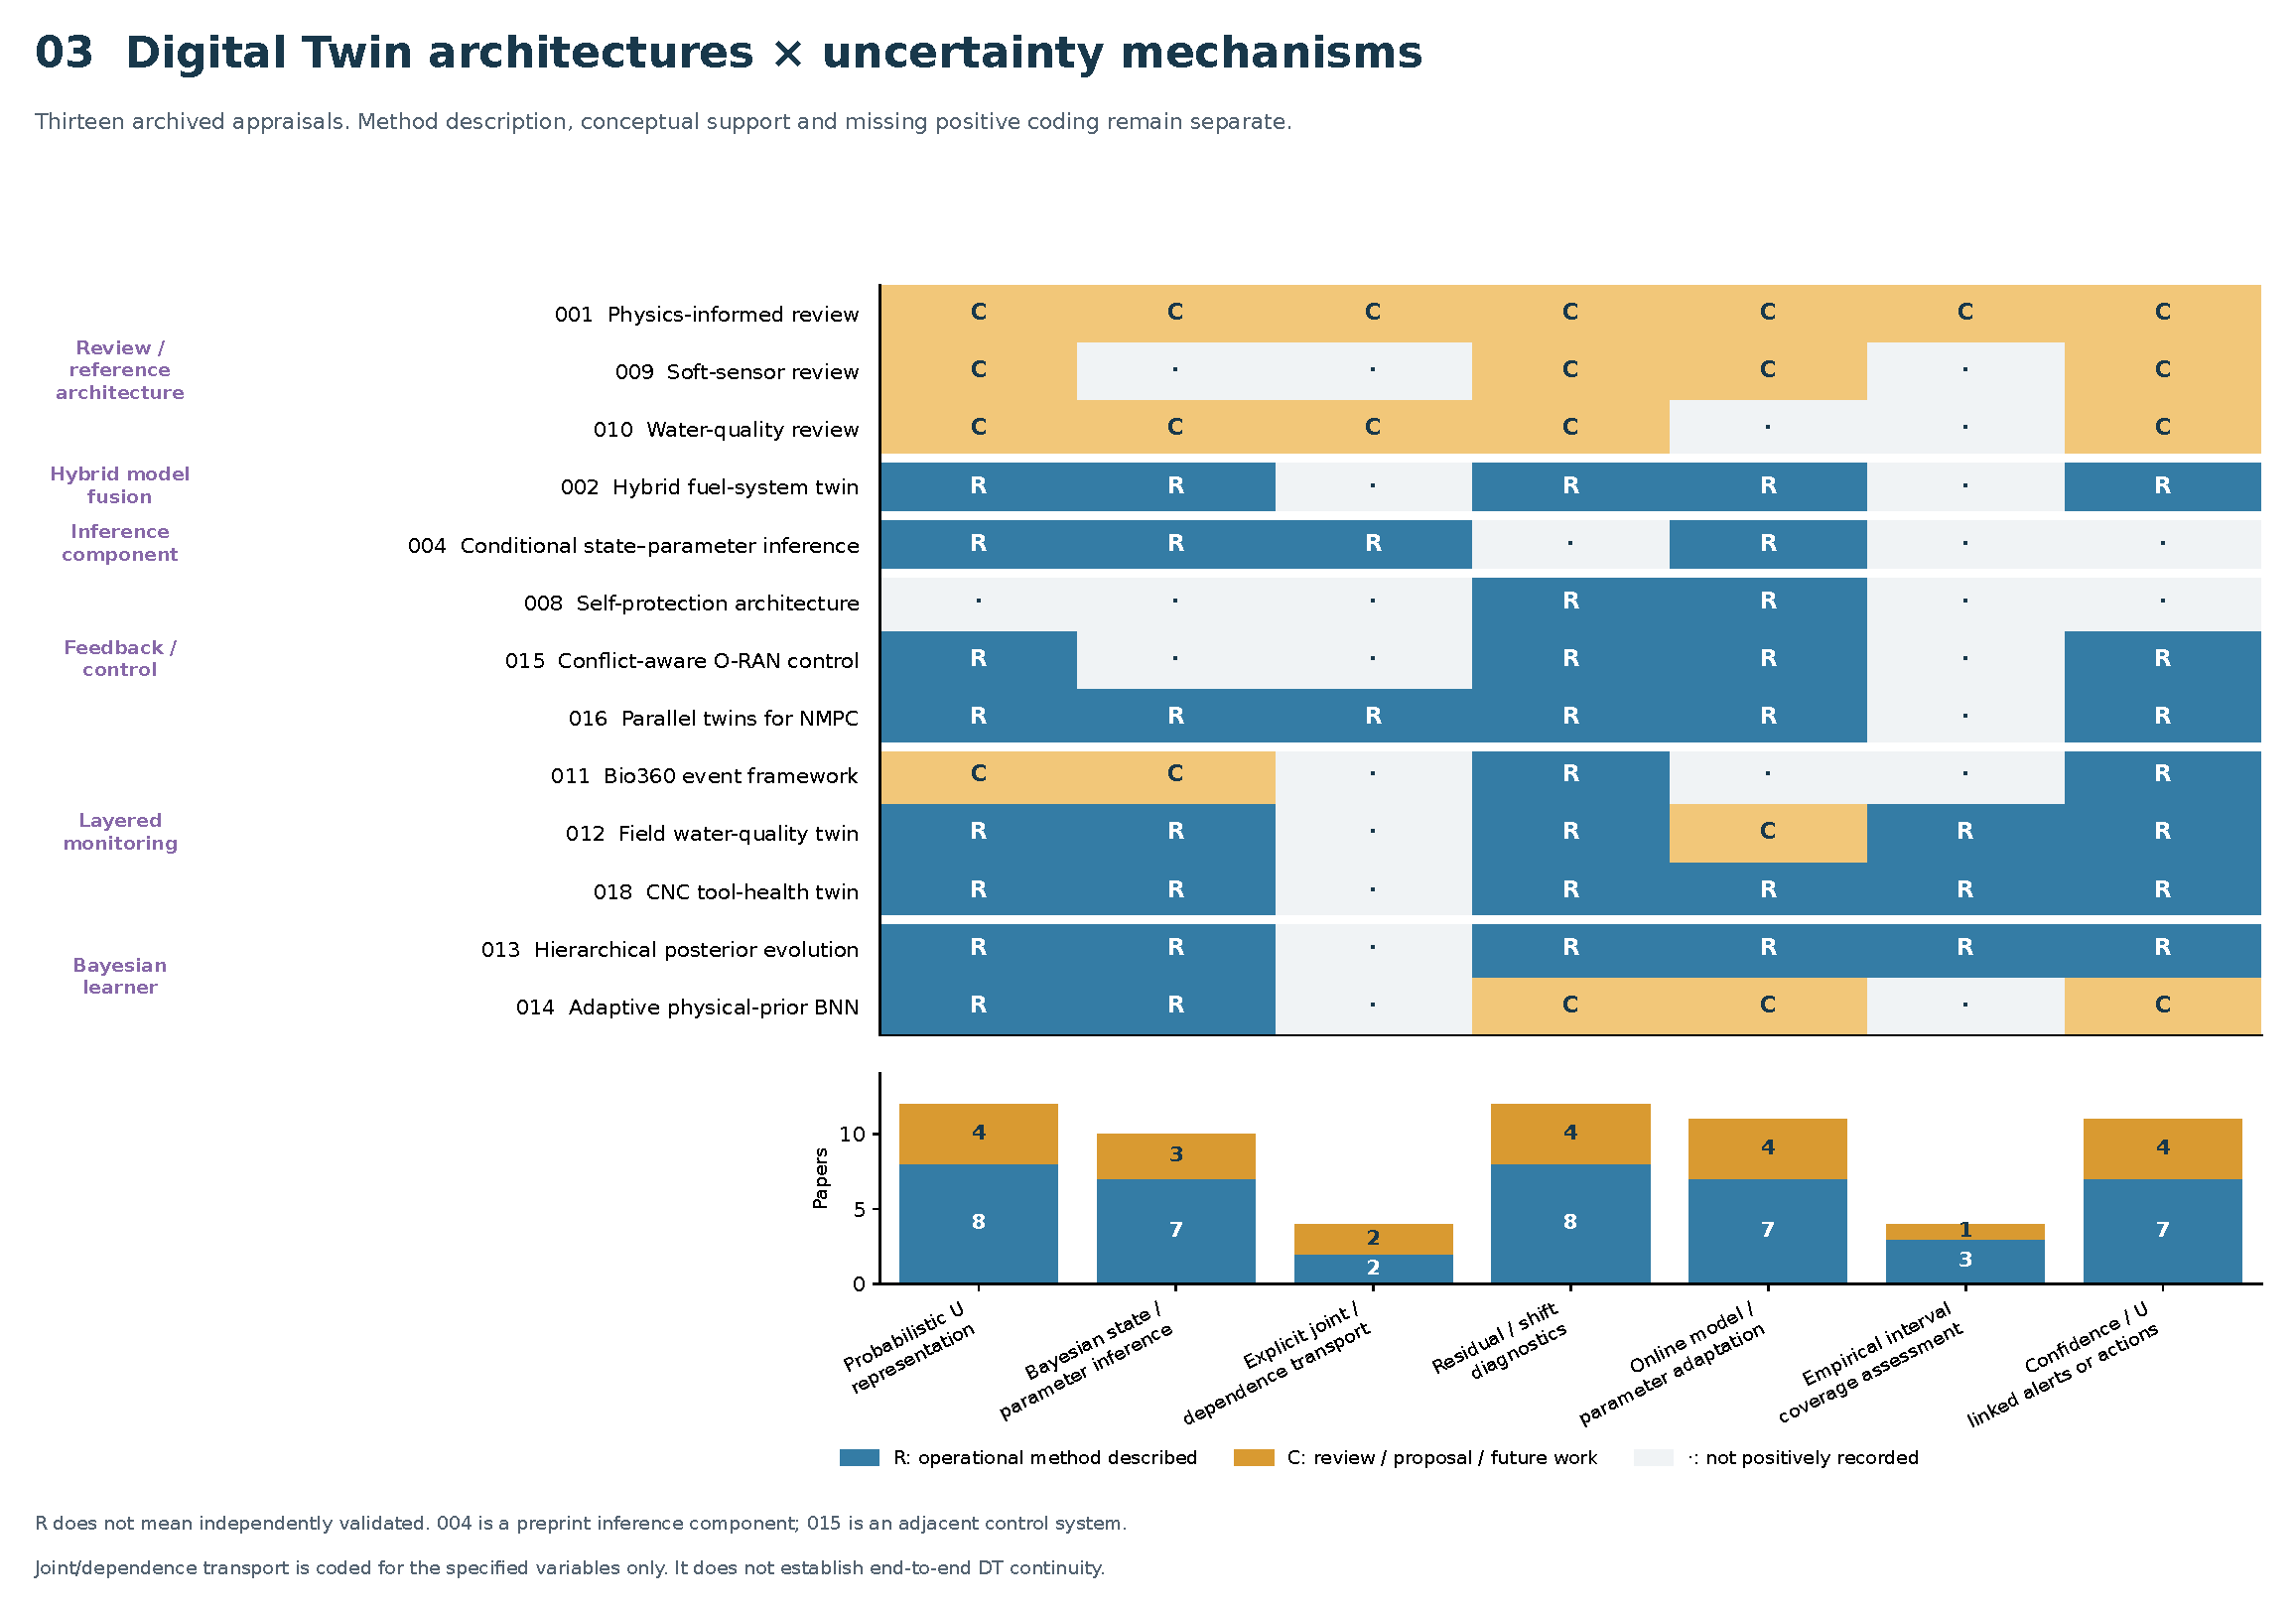
\includegraphics[width=\textwidth]{relational_analysis/results/figures/03_dt_uncertainty_mechanisms.pdf}
\caption{Uncertainty mechanisms across thirteen DT-related appraisals. R denotes an operational method described in the archived extraction; C denotes conceptual, review or prospective support; an unmarked cell has no positive recorded code. Architecture-family labels are reviewer groupings. Dependence-transport codes apply only to the represented variables and do not establish end-to-end continuity.}
\label{fig:relational-dtu}
\end{figure*}

\begin{figure*}[t]
\centering
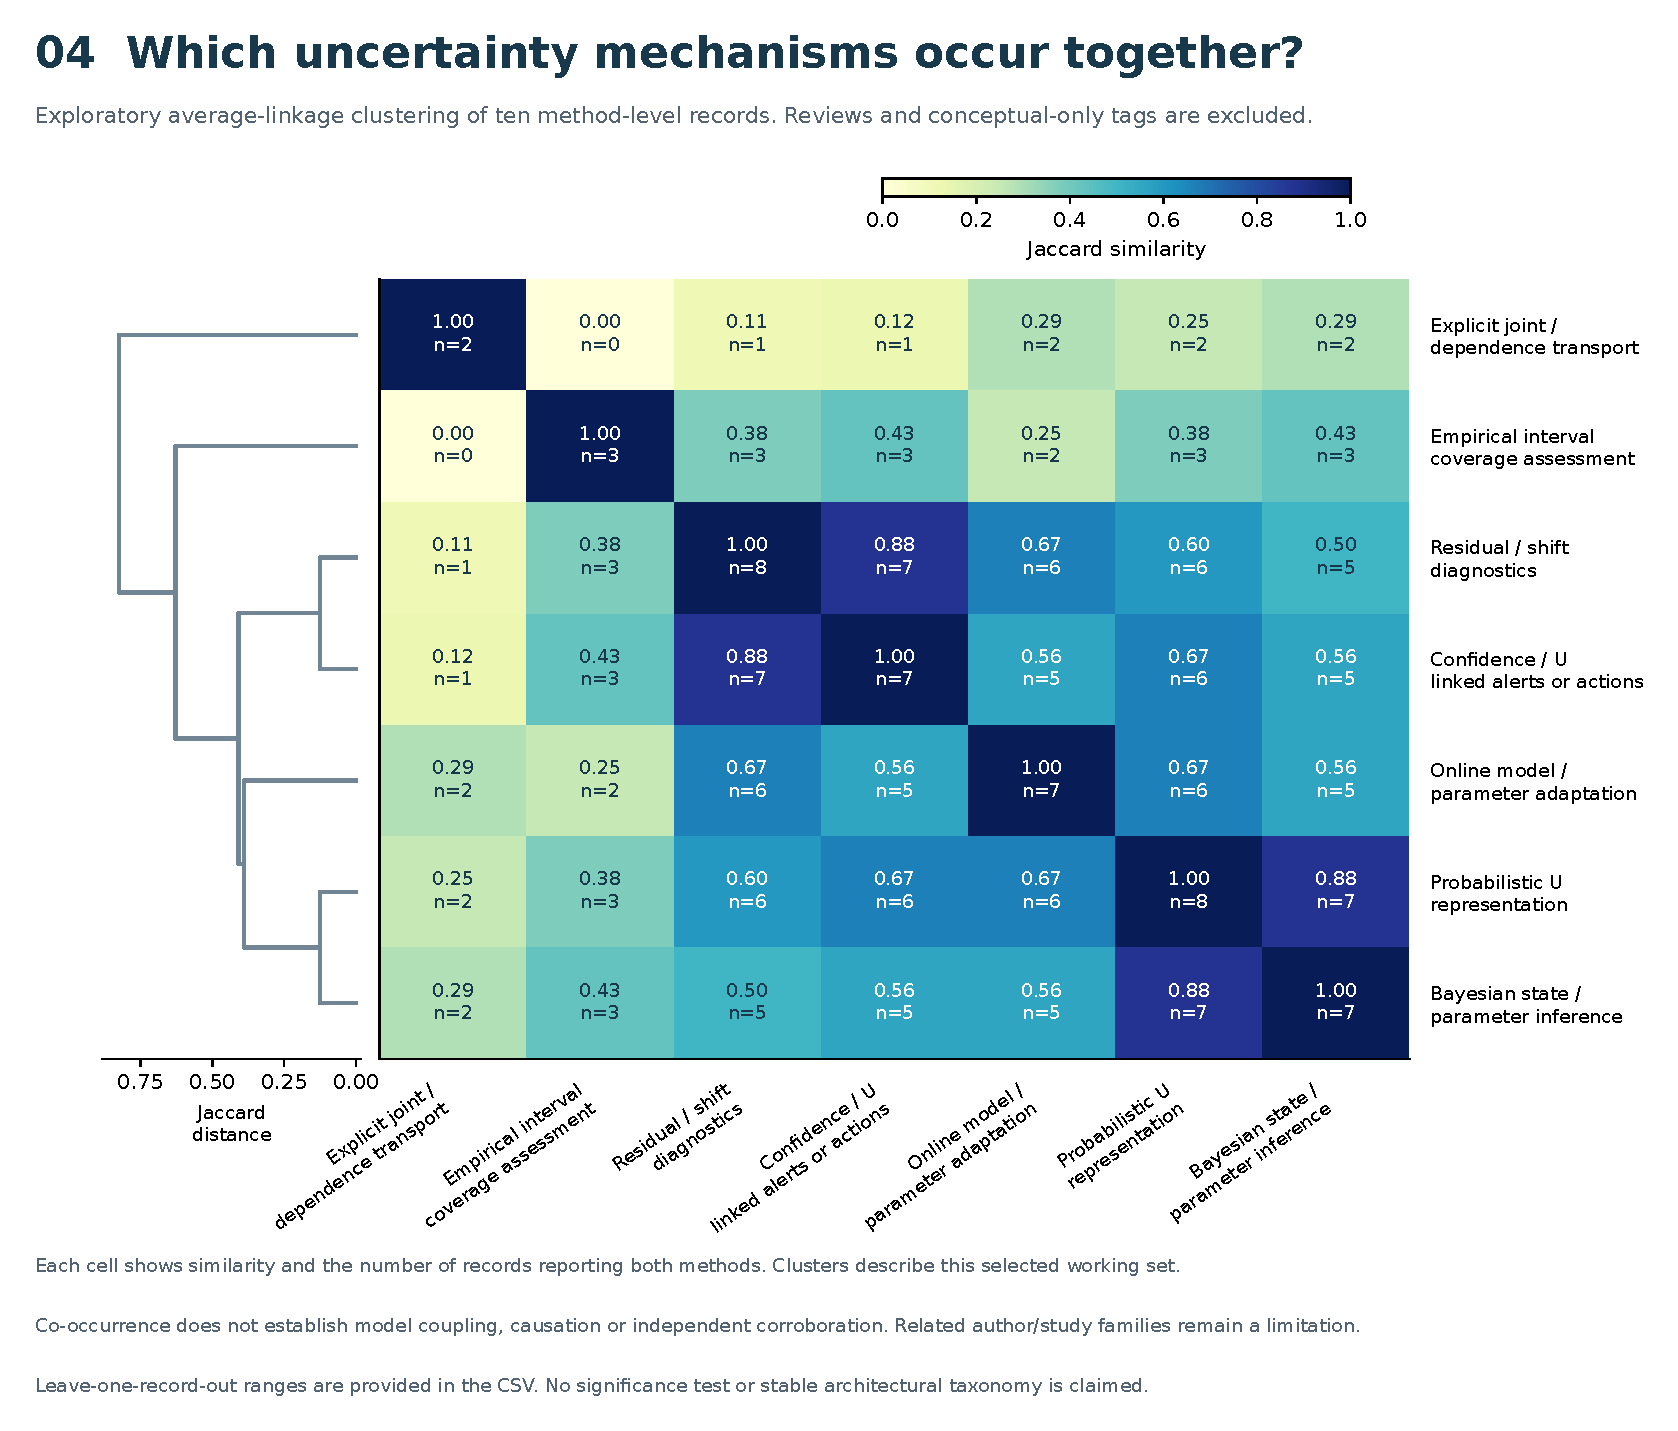
\includegraphics[width=\textwidth]{relational_analysis/results/figures/04_method_cooccurrence.pdf}
\caption{Exploratory mechanism co-occurrence across ten non-review records using only R codes. Each cell gives Jaccard similarity and shared-publication count. Average-linkage clustering uses one minus Jaccard similarity; leave-one-record-out sensitivity ranges accompany the source table. Co-occurrence is not evidence of causal or technical coupling.}
\label{fig:relational-cooccurrence}
\end{figure*}

\begin{figure*}[t]
\centering
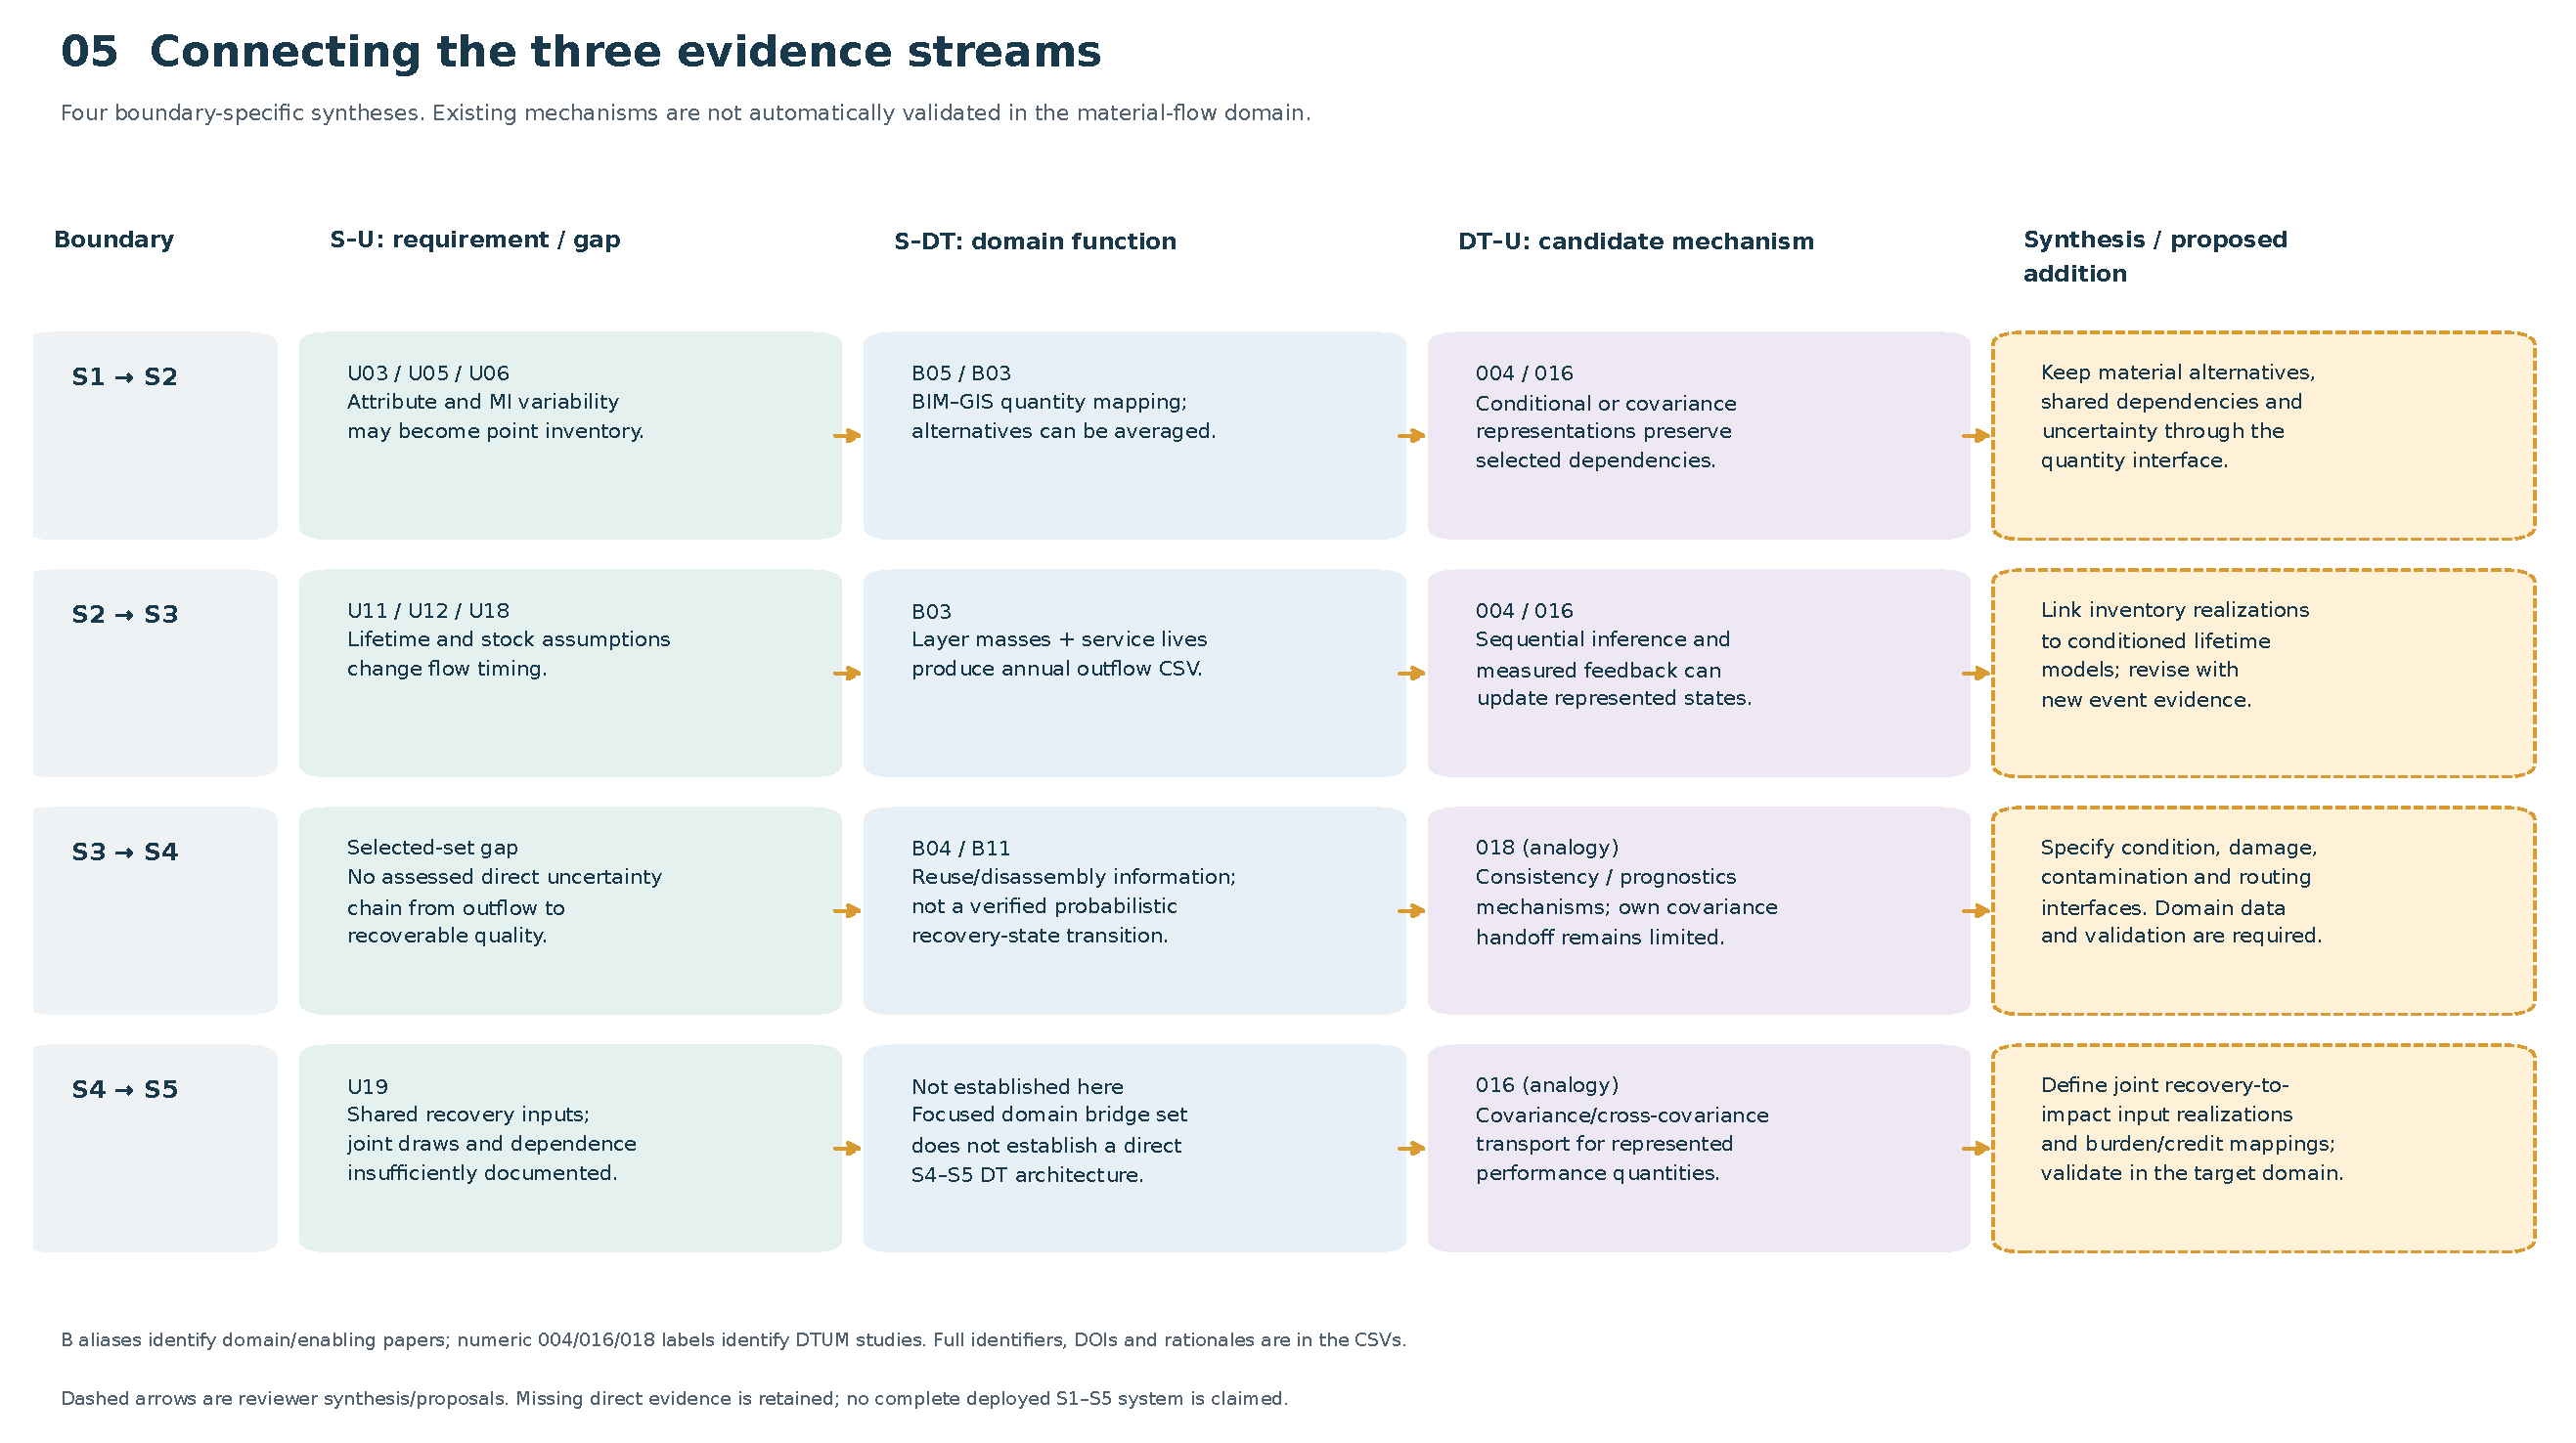
\includegraphics[width=\textwidth]{relational_analysis/results/figures/05_evidence_to_architecture.pdf}
\caption{Four boundary-specific paths connecting uncertainty requirements, domain functions and candidate DT uncertainty mechanisms. Dashed arrows and the final column denote reviewer synthesis or proposed gap responses. Generic mechanisms require compatibility assessment and validation before transfer to material-flow applications.}
\label{fig:relational-paths}
\end{figure*}

\begin{figure*}[t]
\centering
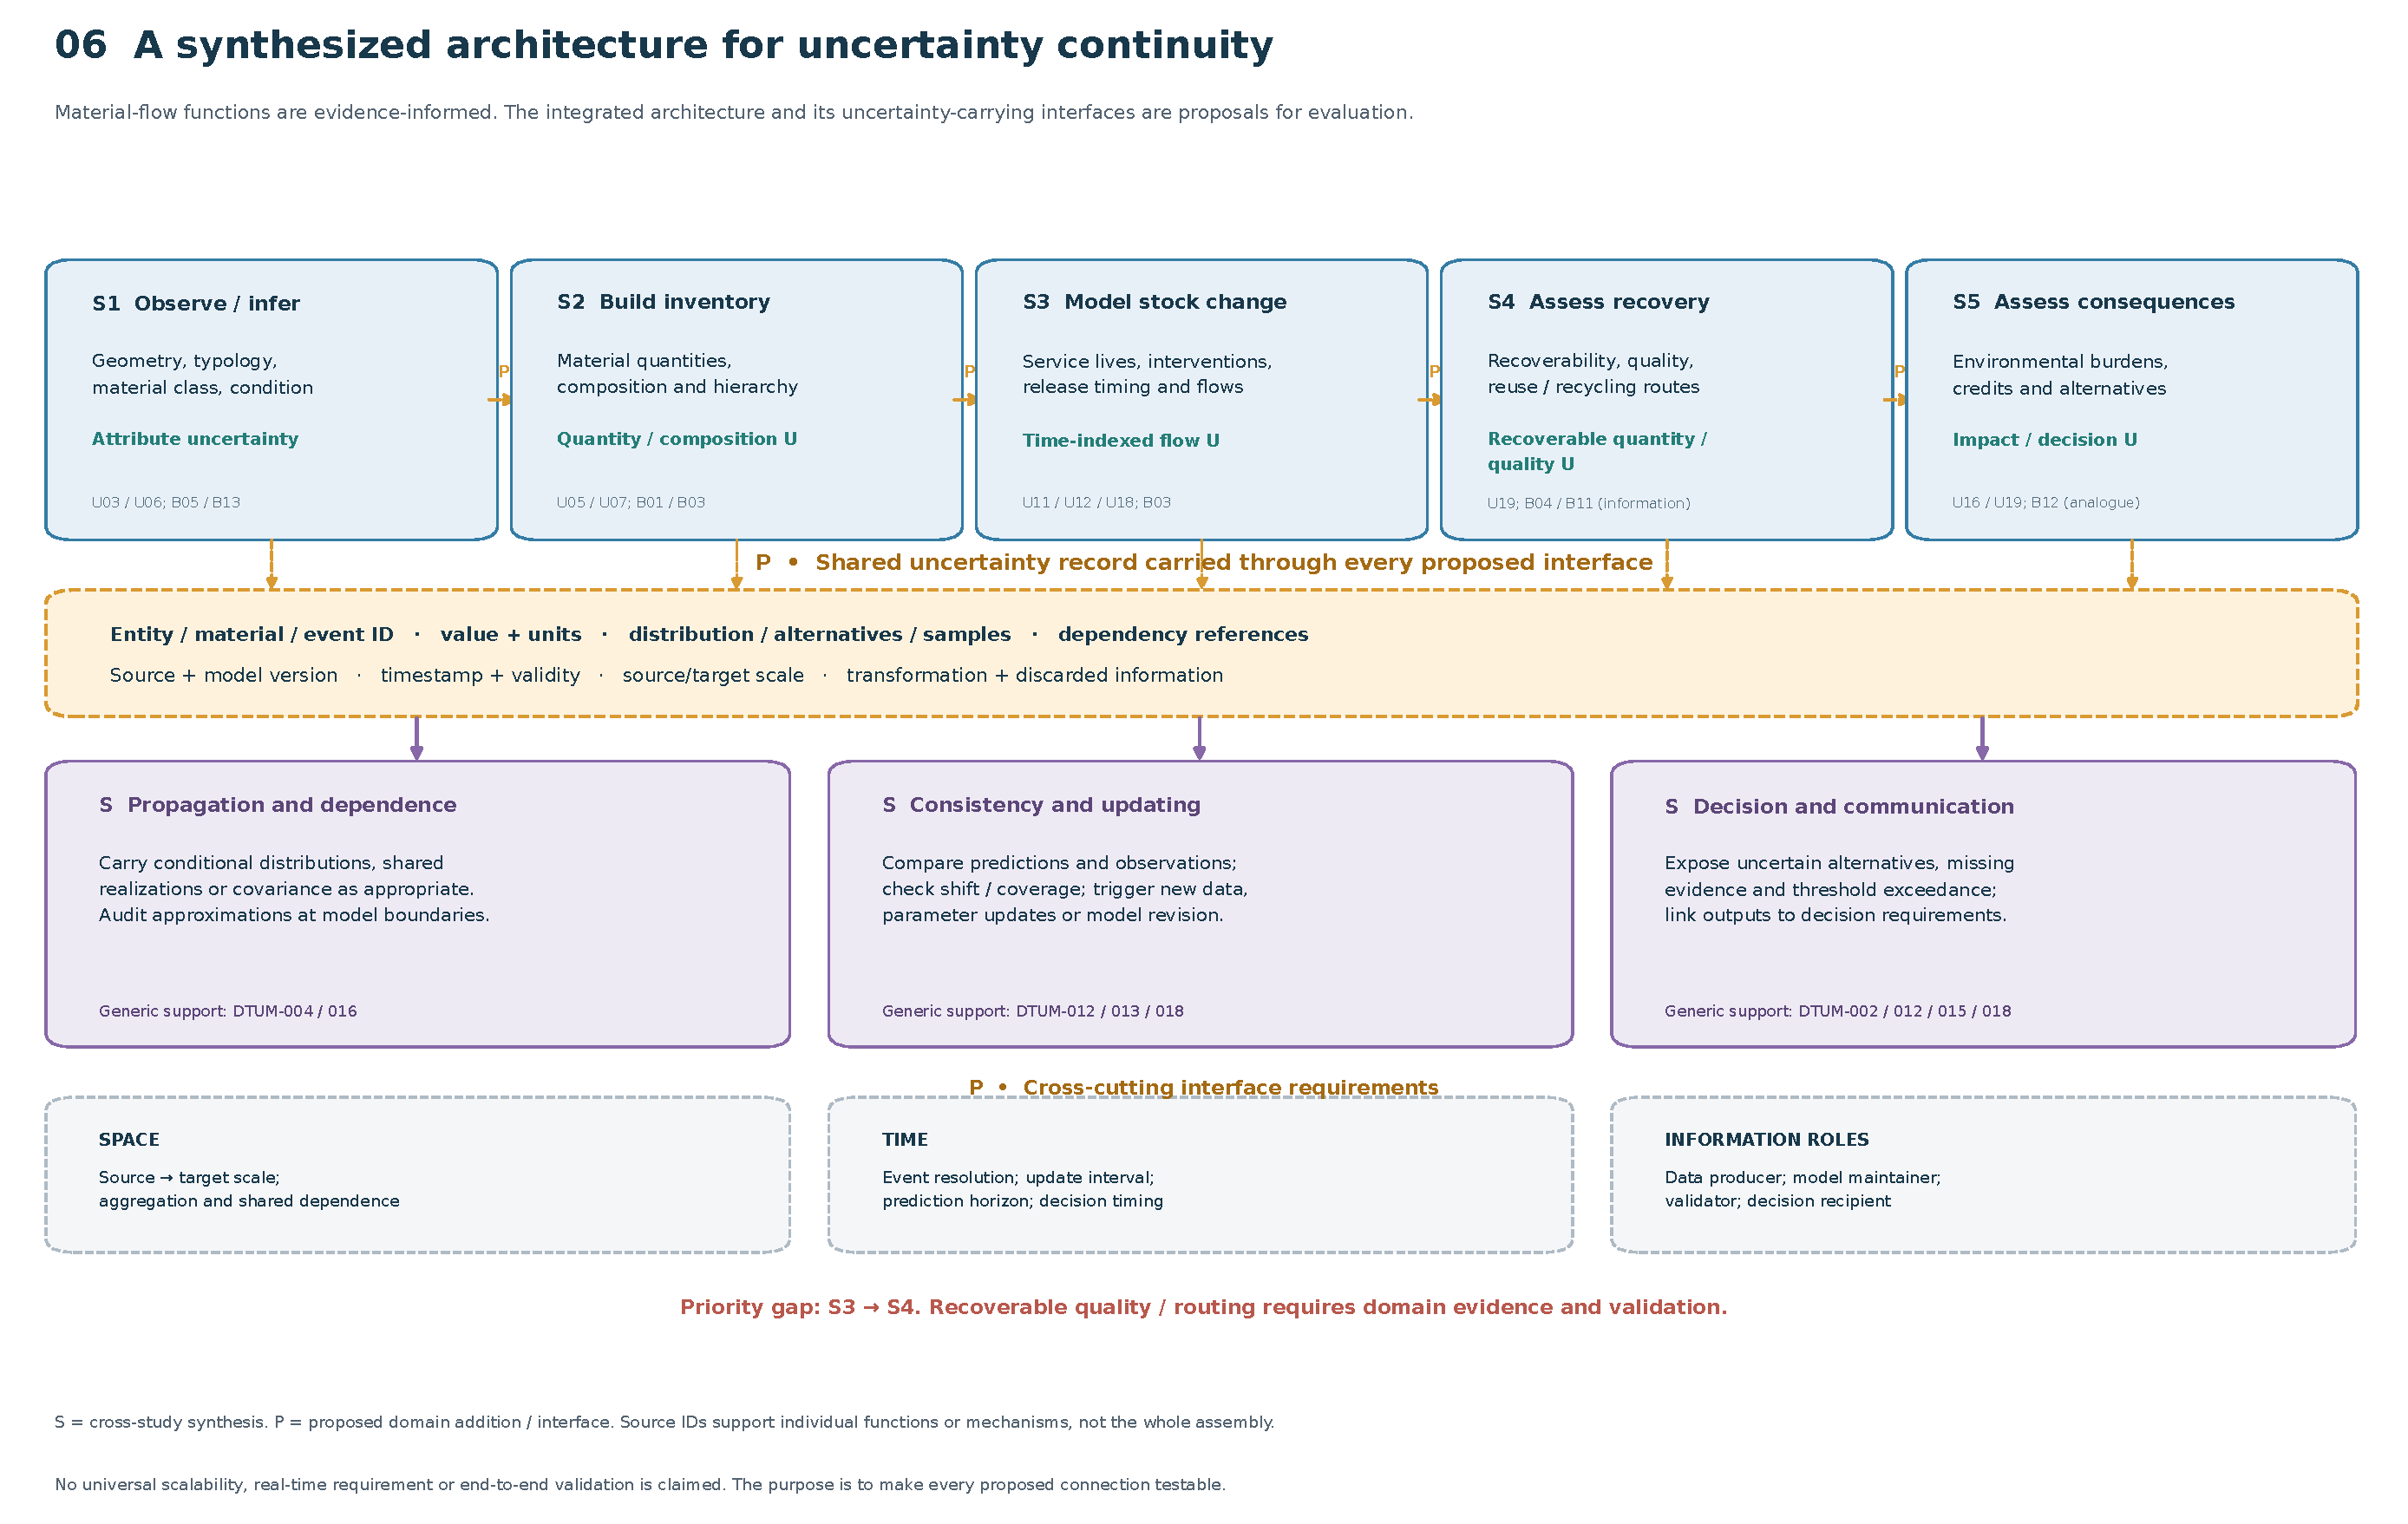
\includegraphics[width=\textwidth]{relational_analysis/results/figures/06_synthesized_architecture.pdf}
\caption{Evidence-informed architecture proposed for uncertainty continuity in circular built-environment material flows. Source identifiers support individual functions and mechanisms, not the assembled system. S denotes cross-study synthesis and P a proposed interface or domain addition. Space, timing and information roles constrain the interfaces; neither universal scalability nor end-to-end validation is claimed.}
\label{fig:relational-architecture}
\end{figure*}
